\hypertarget{electrical-terms-and-components}{%
\section{Electrical Terms and
Components}\label{electrical-terms-and-components}}

In this section, review the concepts of voltage, current and resistance,
as well as some of the basic components. We begin with a common analogy
relating the flow of electricity to water flow. This analogy is probably
over used and has its limitations, but it does help in getting started.
\textbf{Voltage} is the electrical pressure in the circuit. If we use a
water pipe as an analogy, you can think of water pressure in the pipe as
the voltage. The electrical pressure is measured in \texttt{Volts}. The
symbol used in computation is \(v\). \texttt{Current} is the flow of
electrons along a conductor. Again, using the water pipe analogy, think
of water flow in a pipe. The current flow is measured in Amps and the
symbol used is \(i\). \textbf{Resistance} is the measure of the
difficulty to pass an electric current through that element. It is
denoted by \(R\) and measured in units of Ohms. The power in an
electrical circuit is measured in \texttt{Watts} and Watts = Volts *
Amps. About 770 Watts makes up one horsepower. The fundamental
components are given in \texttt{fig:resistor}, \texttt{fig:capacitor},
\texttt{fig:inductor}.

\begin{quote}
\texttt{Resistor} (Ohms): resists the current flow, \(V = iR\) (think of
a narrowing in a pipe (a) Element (b) Resistor circuit diagram.

\texttt{Capacitor} (Farads): stores energy in an electrical field,
\(i = \displaystyle C\frac{dV}{dt}\) (think of a storage tank). (a)
Element (b) Capacitor circuit diagram.

\texttt{Inductor} (Henrys): stores energy in a magnetic field,
\(V = \displaystyle L\frac{di}{dt}\) (think of a flywheel in the pipe.)
(a) Element (b) Inductor circuit diagram.
\end{quote}

\begin{longtable}[]{@{}@{}}
\caption{Resistor color codes}\tabularnewline
\toprule
\endhead
\bottomrule
\end{longtable}

The fundamental law in circuits is \texttt{Ohm’s\ Law},
\texttt{circuitsohmslaw}:

\[V = iR\]

where \(V\) is in volts, \(i\) is in amps, \(R\) is in Ohms.

\begin{quote}
Ohms Law. Note the direction of current flow is the opposite electron
flow.

Using the water metaphor, the water pressure is like voltage, the water
flow is like the current and the narrowing of the pipe is similar to the
resistor (pipe resistance).
\end{quote}

Current flow can be in one direction or vary in direction. These are
known as \texttt{direct\ current} (\texttt{DC}) and
\texttt{alternating\ current} (\texttt{AC}).

\begin{figure}
\centering
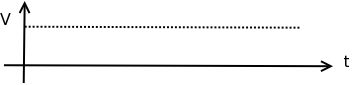
\includegraphics[width=0.6\textwidth,height=\textheight]{ElectricalFigures/dc.*}
\caption{Direct current.}
\end{figure}

\begin{figure}
\centering
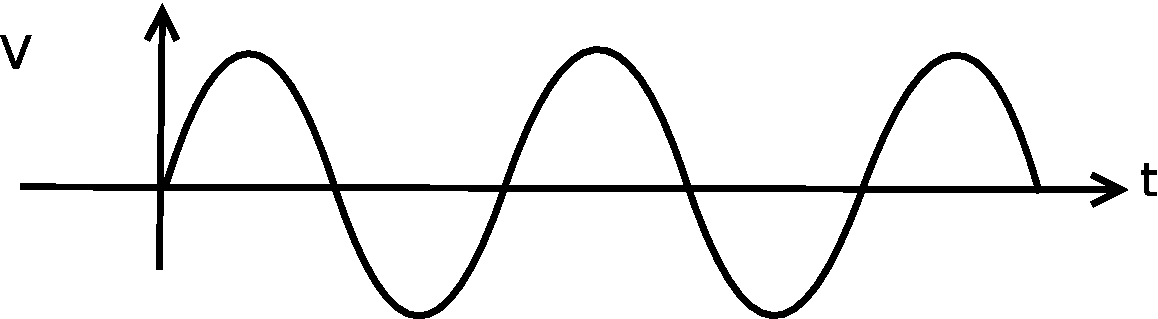
\includegraphics[width=0.6\textwidth,height=\textheight]{ElectricalFigures/ac.*}
\caption{Alternating current.}
\end{figure}

Electronic devices run on direct current and this is the type of power
delivered by batteries. Large scale power distribution is most
efficiently done using alternating current (and at much higher
voltages). So the power that enters our homes is AC. To get alternating
current down from the high voltage levels that are used in transmission
lines to an outlet, a transformer is used. You have often heard them as
they make that characteristic hum. To convert from AC to DC, another
approach is used. A device called a diode has the property that it
allows current to flow one way, in essence it is an electrical one way
valve, \texttt{circuitdiode}.

\begin{quote}
\texttt{Diode}.

The change in the current flow after the diode.
\end{quote}

A clever connection of four diodes known as a diode bridge reroutes
current so that it flows in one direction only (will still vary, but at
least stay the same direction), \texttt{circuitdiodebridge}. This bridge
can also be used to protect inputs to electronic devices in case
positive and negative lines get reversed.

\begin{quote}
A combination of diodes known as a bridge to convert alternating current
into positive current.
\end{quote}

\begin{figure}
\centering
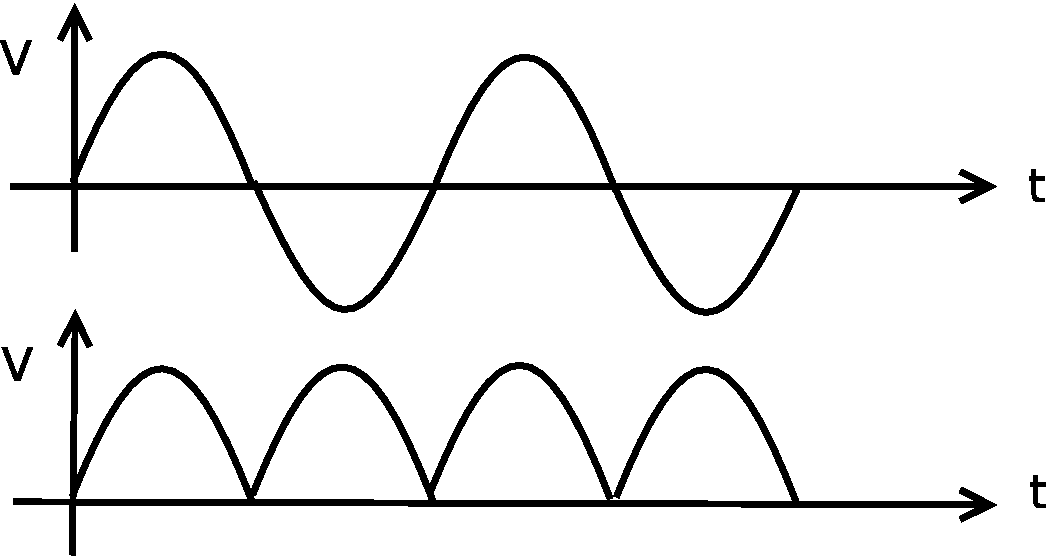
\includegraphics[width=0.6\textwidth,height=\textheight]{ElectricalFigures/acdc.*}
\caption{The change in the current flow after the bridge circuit.}
\end{figure}

The current headed out of the diode bridge flows in one direction, but
the voltage is still fluctuating. Another device is employed, a
capacitor. Using the water analogy, think of the capacitor as a storage
tank. It will smooth out the voltage fluctuations like a pond smooths
out stream flow. These basic circuit devices are used in a common
household circuits such as a power supply, \texttt{powersupply}.

\begin{quote}
The power supply circuit to provide a fixed 5 volts.
\end{quote}

In this circuit, wall power (alternating current at 115 volts) is fed
into the left side. S1 is the symbol for the on/off switch. The next
device is a 3 Amp (3A) fuse. The high voltage AC is fed into the
transformer (T1) and dropped down to 24 volts (still AC). Next comes the
bridge circuit which re-routes the current flow so we have rectified (or
unidirectional) current flow. Following the bridge is a large capacitor
that will smooth the flow. It still has ripples in the flow (and they
can be large). So the current is fed into a voltage regulator which
significantly smooths the voltage level. The resistors and capacitors
surrounding the regulator (LM317) select the output voltage level. Now
you understand what is inside those bricks that charge your laptop,
phone, camera, etc.

\hypertarget{batteries}{%
\section{Batteries}\label{batteries}}

Most mobile devices rely on batteries and they will be the main power
source for the robots we discuss. {[}It is possible to have solar
powered or inductively powered systems and maybe we will see more of
this in the future.{]} All batteries are relatively slow, controlled,
chemical reactions. They are not devices that store electric charge. The
closest thing to that is a capacitor, which is comprised of two metal
plates with an insulator between them. By applying voltage, you charged
the plates, storing energy in the form of actual electric charge.
However, capacitors tend to discharge all of their stored energy at
once. In addition, the total energy they can store is far less than most
batteries. Batteries, on the other hand, store energy in the form of
chemical potential energy. This is far more stable than storing raw
electric charge, but it does lead to a few problems. The big one is
that, since the energy storage relies on chemistry, temperature is
important. Being stored in a place that is too hot or too cold can cause
a battery to burst, or drain it. Another is that, over time, the
chemicals will degrade or react with other chemicals, causing the
battery's maximum storage potential to decline.

We normally divide batteries up into Primary (non-rechargeable) and
Secondary (rechargable) chemistries. We will briefly discuss secondary
chemistries. There are three well known currently used chemistries for
rechargeable batteries: Lead-Acid, Nickel Metal Hydride (NiMH), Lithium
Polymer (LiPo). Lead-Acid is the type found in automobile, boat,
motorcycle batteries.

\begin{quote}
Batteries: a) \texttt{Lead-Acid\ cell}. b) \texttt{Li-Po} c) Battery
circuit symbol.

\begin{longtable}[]{@{}llll@{}}
\toprule
\begin{minipage}[b]{0.22\columnwidth}\raggedright
Chemistry:\strut
\end{minipage} & \begin{minipage}[b]{0.15\columnwidth}\raggedright
Lead-Acid\strut
\end{minipage} & \begin{minipage}[b]{0.23\columnwidth}\raggedright
NiMH\strut
\end{minipage} & \begin{minipage}[b]{0.23\columnwidth}\raggedright
LiPo\strut
\end{minipage}\tabularnewline
\midrule
\endhead
\begin{minipage}[t]{0.22\columnwidth}\raggedright
Cell:\strut
\end{minipage} & \begin{minipage}[t]{0.15\columnwidth}\raggedright
2.1V\strut
\end{minipage} & \begin{minipage}[t]{0.23\columnwidth}\raggedright
1.2V\strut
\end{minipage} & \begin{minipage}[t]{0.23\columnwidth}\raggedright
3.7 V\strut
\end{minipage}\tabularnewline
\begin{minipage}[t]{0.22\columnwidth}\raggedright
Weight:\strut
\end{minipage} & \begin{minipage}[t]{0.15\columnwidth}\raggedright
Heavy\strut
\end{minipage} & \begin{minipage}[t]{0.23\columnwidth}\raggedright
Light\strut
\end{minipage} & \begin{minipage}[t]{0.23\columnwidth}\raggedright
Light\strut
\end{minipage}\tabularnewline
\begin{minipage}[t]{0.22\columnwidth}\raggedright
Energy density:\strut
\end{minipage} & \begin{minipage}[t]{0.15\columnwidth}\raggedright
Moderate\strut
\end{minipage} & \begin{minipage}[t]{0.23\columnwidth}\raggedright
High\strut
\end{minipage} & \begin{minipage}[t]{0.23\columnwidth}\raggedright
Very high\strut
\end{minipage}\tabularnewline
\begin{minipage}[t]{0.22\columnwidth}\raggedright
Environment:\strut
\end{minipage} & \begin{minipage}[t]{0.15\columnwidth}\raggedright
Toxic\strut
\end{minipage} & \begin{minipage}[t]{0.23\columnwidth}\raggedright
Relatively green\strut
\end{minipage} & \begin{minipage}[t]{0.23\columnwidth}\raggedright
Relatively green\strut
\end{minipage}\tabularnewline
\bottomrule
\end{longtable}
\end{quote}

\hypertarget{battery-voltage}{%
\subsection{Battery Voltage}\label{battery-voltage}}

We'll start with voltage because that's the easiest one to handle. You
want to make sure the voltage your batteries produces matches the
voltage rating for the things you want to power: motors, cpu, sensors,
etc. However, there's another consideration to make. You almost never
want your batteries directly connected to your sensitive electronics.
You always want a regulator of some sort in between. Why? As you drain a
battery, the voltage will decline over time. In addition, large loads on
the battery can temporarily cause the voltage to fluctuate i.e. powering
motors. Motors also cause back-emf, but we'll talk about that later. All
of this can cause damage to unshielded electronics. In addition to the
power fluctuations, you rarely have motors that you want to drive with
the same voltage as the computer. In practice, you'll want to match your
main battery voltage to the voltage of the motors you want to power, and
then use regulators to smooth and reduce the voltage for the other
components.

\hypertarget{battery-capacity---mah-milli-amp-hours}{%
\subsection{Battery Capacity - mAh ``milli-Amp
Hours''}\label{battery-capacity---mah-milli-amp-hours}}

This is a measure of how much actual energy the battery can hold. To put
it simply, a 1000mAh battery could sustain a drain of 1A for 1 hour
before being depleted. If you draw 2A it will only last half an hour. At
0.5A, two hours.

\hypertarget{the-c-rating}{%
\subsection{The C rating}\label{the-c-rating}}

Most batteries have a C rating. This is a somewhat cryptic value that
tells you how quickly a battery can discharge without damaging itself.
This is not a limit on how much current the battery can draw. Ohm's law
will dictate the current that gets drawn from the battery. The C rating
just tells you what is safe. The tricky bit is that the actual safe rate
of discharge depends on the size of the battery. Here's the simple way
to think about it. The amount of continuous current drain a battery can
handle without damaging itself is obtained by multiplying the C rating
with the battery capacity. For instance, a 1500mAh battery with a 5C
rating can handle a continuous drain of 30,000mA or 30A.

\hypertarget{lead-acid-batteries---pb}{%
\subsection{Lead Acid Batteries - Pb}\label{lead-acid-batteries---pb}}

Lead acid batteries are very stable which is why we use them in cars.
They also have a pretty good capacity, and are able to source a
tremendous amount of current at once. This is good, because it takes a
lot of force to turn over an engine. For a rugged, outdoor robot that
may experience a variety of temperature conditions, lead-acid may be the
way to go. However, lead-acid batteries are generally larger and heavier
than their counterparts. Charging them is easy. Just hook them up to a
power supply, set the power supply to the battery's rated voltage, and
limit the current. What you limit the current to depends on the battery.
Car batteries can generally handle up to 6A. The real problem is heat.
If you charge too fast, the metal plates in the battery heat up, and can
cause the acid to boil. This creates potentially toxic vapors and, if
the vapors escape the battery housing, reduce the lifespan and charge of
the battery. Other than charging too quickly, there isn't much to worry
about here. Please charge in a well-ventilated area, just in case.
Running a lead-acid battery dead isn't really a big deal as long as you
don't leave it dead for a long time, or it doesn't get too cold while
dead.

\hypertarget{lithium-polymer---lipo}{%
\subsection{Lithium Polymer - LiPo}\label{lithium-polymer---lipo}}

Lithium Polymers are light-weight, small, and can store a great deal of
power. A LiPo battery generally consists of some number of cells. Each
cell has a rated voltage of 3.7V. Batteries with more voltage are built
by putting multiple cells in series. This voltage has to do with the
internal chemistry. LiPo batteries are not nearly as stable as lead
acid. There are three major concerns when dealing with a LiPo. First,
only charge using a LiPo charger. There are some extra pins on a LiPo
battery that tell the charger important information about the cells
within. Second, make sure you look up the rating for charging a LiPo.
The general rule of thumb is that a LiPo can be charged at the rate of
1C. Charging it slower is fine. Charging faster can cause the LiPo to
heat up, swell, and potentially burst. When the LiPo bursts, the
chemicals inside will spontaneously burn, creating fire, pressure, and
heat. Third, never ever cut or puncture a LiPo. A ruptured LiPo is not
safe and has caused serious fires.

That all said, LiPo batteries are pretty safe if you follow the
guidelines for charging. There are two more things to worry about. 3.7V
is the rated voltage for a cell, but when you charge, you generally
charge to about 4.2V - the charger will handle this. Never overcharge
the LiPo. However, unlike a lead-acid battery, letting the charge get
too low in a LiPo will permanently damage it. The minimum safe level for
a single cell is 3V. Always monitor the voltage of LiPo batteries you
are using and ensure they don't drop below this level. The difficult
part is, LiPo voltage doesn't drop linearly. \texttt{fig:lipovoltage}
shows voltage versus charge for a LiPo. As you can see from the graph,
you have to monitor the battery voltage very carefully, because it
decreases rapidly once the charge gets low.

\begin{quote}
LiPo Voltage VS Charge.
\end{quote}

As a side note, this chart is for one specific battery I found on a
forum post at Traxxas.com. Individual results may vary in specifics, but
the point is the same. Monitor your voltage and don't let it drop below
3.0V per cell. There is one additional caveat. LiPo batteries don't hold
their charge forever, and they will, if left sitting on a shelf for long
periods of time, eventually degrade. It is recommended to discharge and
charge a LiPo battery every few months when it is not in active use.
Discharging can be done by using the LiPo while closely monitoring the
voltage, or with a dedicated charger.

The final thing to mention is balancing. Because a LiPo battery may be
made up of multiple cells, the total voltage isn't enough to tell the
health of the battery. Some chargers will also balance while they
charge. Balancing slowly bleeds charge from one cell and puts it into
another cell. This keeps the cells from becoming unbalanced. This is a
good thing since often each cell will discharge differently. This can
lead to one cell with a much higher or lower voltage than the others. If
one cell gets overcharged, it may swell and/or rupture. If one cell gets
too low, it may ``die''. Dead cells are ones that have dropped to a low
enough voltage that they cannot safely be recharged. Most chargers will
refuse to charge the battery if there are dead cells. If you know what
you're doing, sometimes dead cells can be nursed back to life, but it's
a delicate and potentially dangerous procedure. It's usually better to
recycle the battery and get a new one.

\hypertarget{other-batteries}{%
\subsection{Other Batteries}\label{other-batteries}}

There are three more common types of batteries. Lithium Iron Phosphate
-LiFePO4 often pronounced ``LieFo'' - Nickel Metal Hydride - NiMH - and
Nickel Cadmium - NiCd pronounced ``Nigh-Cad''. Roughly, LiFePO4 are
similar to LiPo batteries but more stable and more expensive.

\hypertarget{tips-for-not-lighting-things-on-fire}{%
\subsection{Tips For Not Lighting Things On
Fire}\label{tips-for-not-lighting-things-on-fire}}

Forethought and attentiveness are key for keeping the magic smoke inside
the components. All electrical components are made using plastic,
silicon, some trace metals, and a mystical substance called magic smoke.
If you give the component too much voltage, current, or heat the magic
smoke will use this extra energy to break free and escape. It is a very
clever substance, and even just a momentary spike is enough to free it.
At this point the component will no longer work. Nobody is perfect, but
here are a few tips picked up over the years to keep the magic smoke
locked up tight.

\hypertarget{turn-off-the-power}{%
\subsubsection{Turn Off The Power}\label{turn-off-the-power}}

This should be common sense, but you'd be surprised how often people get
overconfident about what they're doing and modify a circuit while it's
powered. Sure, if you know what you're doing you're theoretically safe
but in practice it is foolish and dangerous. The problem arises when one
of those tiny wires gets away from you or if you drop a metal piece or
if you touch something by accident or ... Powered wires appear to be
supernaturally attracted to conductive terminals, particularly ones that
will causes sparks. Just don't do it. The five seconds it takes to flip
off the power could save you three days of waiting for new parts or a
visit to the emergency room.

\hypertarget{electrical-tape}{%
\subsubsection{Electrical Tape}\label{electrical-tape}}

If you're working on a circuit and if you aren't immediately dealing
with a wire, tape the end. Most of the instances in which folks blew
something up was because they forgot about a wire that wasn't connected,
and it brushed up against something else, making a short. This is
particularly important when dealing with batteries. Remember, you can't
turn a battery off. If both terminals of a battery aren't connected to
something, the free wires should be taped over. Also, NEVER cut more
than one battery cable at a time. This can short the battery and again
release the magic smoke.
